\documentclass[tikz,border=10pt]{standalone}
\usepackage{amsmath}
\usetikzlibrary{positioning}

\begin{document}
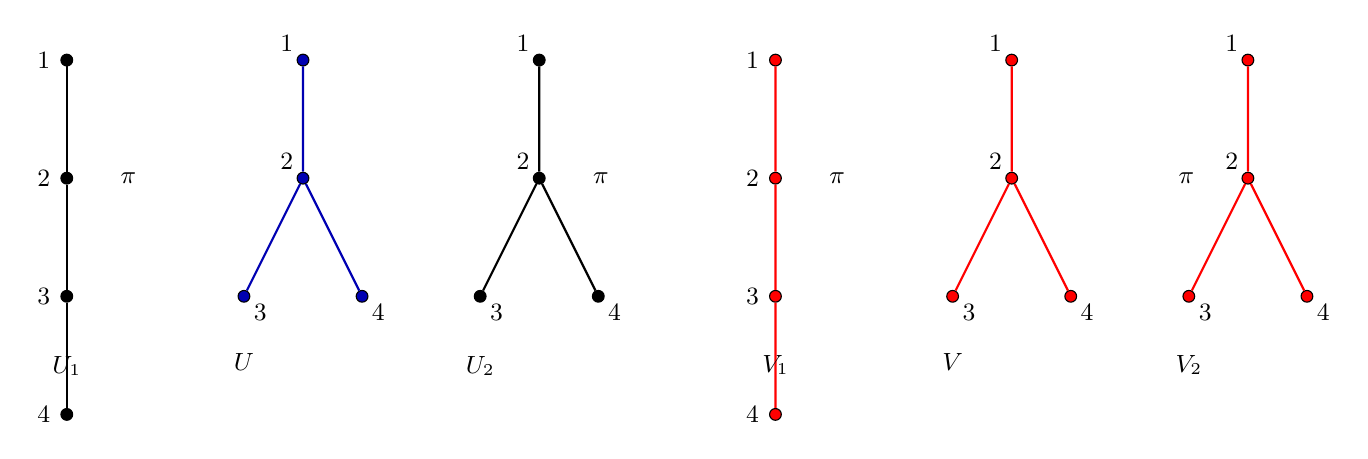
\begin{tikzpicture}[scale=1.5, every node/.style={circle, inner sep=1.5pt}, font=\small]

% Define styles
\tikzset{
    vertex/.style={fill, draw, circle, inner sep=1.5pt},
    redvertex/.style={fill=red, draw, circle, inner sep=1.5pt},
    bluevertex/.style={fill=blue!70!black, draw, circle, inner sep=1.5pt},
    edge/.style={thick, draw}
}

% Leftmost tree U_1
\node[vertex, label=left:{1}] (u1-1) at (0,3) {};
\node[vertex, label=left:{2}] (u1-2) at (0,2) {};
\node[vertex, label=left:{3}] (u1-3) at (0,1) {};
\node[vertex, label=left:{4}] (u1-4) at (0,0) {};

\draw[edge] (u1-1) -- (u1-2);
\draw[edge] (u1-2) -- (u1-3);
\draw[edge] (u1-3) -- (u1-4);

\node[right=0.5cm of u1-2] {$\pi$};
\node[below=0.5cm of u1-3] {$U_1$};

% Middle-left tree U
\node[bluevertex, label=above left:{1}] (u-1) at (2,3) {};
\node[bluevertex, label=above left:{2}] (u-2) at (2,2) {};
\node[bluevertex, label=below right:{3}] (u-3) at (1.5,1) {};
\node[bluevertex, label=below right:{4}] (u-4) at (2.5,1) {};

\draw[edge, blue!70!black] (u-1) -- (u-2);
\draw[edge, blue!70!black] (u-2) -- (u-3);
\draw[edge, blue!70!black] (u-2) -- (u-4);

\node[below=0.5cm of u-3] {$U$};

% Middle-right tree U_2
\node[vertex, label=above left:{1}] (u2-1) at (4,3) {};
\node[vertex, label=above left:{2}] (u2-2) at (4,2) {};
\node[vertex, label=below right:{3}] (u2-3) at (3.5,1) {};
\node[vertex, label=below right:{4}] (u2-4) at (4.5,1) {};

\draw[edge] (u2-1) -- (u2-2);
\draw[edge] (u2-2) -- (u2-3);
\draw[edge] (u2-2) -- (u2-4);

\node[right=0.5cm of u2-2] {$\pi$};
\node[below=0.5cm of u2-3] {$U_2$};

% Rightmost tree V_1
\node[redvertex, label=left:{1}] (v1-1) at (6,3) {};
\node[redvertex, label=left:{2}] (v1-2) at (6,2) {};
\node[redvertex, label=left:{3}] (v1-3) at (6,1) {};
\node[redvertex, label=left:{4}] (v1-4) at (6,0) {};

\draw[edge, red] (v1-1) -- (v1-2);
\draw[edge, red] (v1-2) -- (v1-3);
\draw[edge, red] (v1-3) -- (v1-4);

\node[right=0.5cm of v1-2] {$\pi$};
\node[below=0.5cm of v1-3] {$V_1$};

% Middle-right tree V
\node[redvertex, label=above left:{1}] (v-1) at (8,3) {};
\node[redvertex, label=above left:{2}] (v-2) at (8,2) {};
\node[redvertex, label=below right:{3}] (v-3) at (7.5,1) {};
\node[redvertex, label=below right:{4}] (v-4) at (8.5,1) {};

\draw[edge, red] (v-1) -- (v-2);
\draw[edge, red] (v-2) -- (v-3);
\draw[edge, red] (v-2) -- (v-4);

\node[below=0.5cm of v-3] {$V$};

% Rightmost tree V_2
\node[redvertex, label=above left:{1}] (v2-1) at (10,3) {};
\node[redvertex, label=above left:{2}] (v2-2) at (10,2) {};
\node[redvertex, label=below right:{3}] (v2-3) at (9.5,1) {};
\node[redvertex, label=below right:{4}] (v2-4) at (10.5,1) {};

\draw[edge, red] (v2-1) -- (v2-2);
\draw[edge, red] (v2-2) -- (v2-3);
\draw[edge, red] (v2-2) -- (v2-4);

\node[left=0.5cm of v2-2] {$\pi$};
\node[below=0.5cm of v2-3] {$V_2$};

\end{tikzpicture}
\end{document}